\section{Background and Motivation}
\label{background}

\begin{figure}
	\centering
	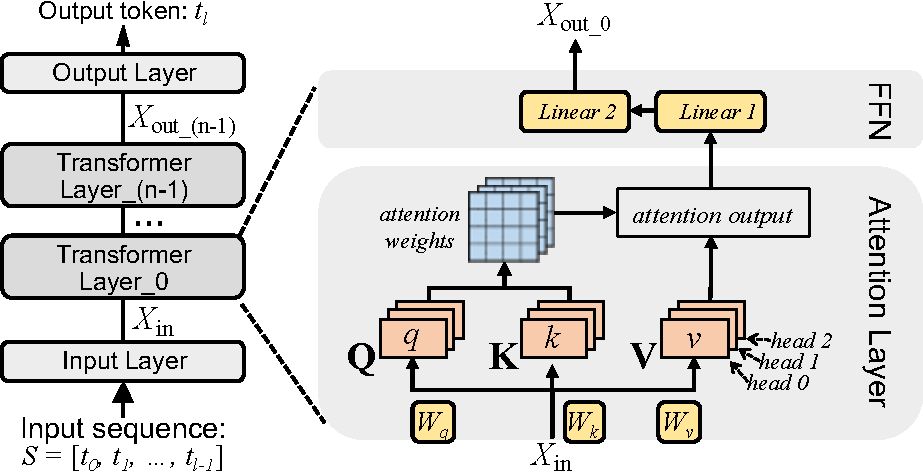
\includegraphics[width=3.4in, height=1.6in]{transformer.pdf}
	\vspace{-0.05in}
	\caption{The LLM model structure.}
	\label{fig:llm}
	\vspace{-0.1in}
\end{figure}

\subsection{Large Language Model Basics}
\label{sec:llm-basic}


%A generative LLM typically consists of an input layer, tens of consecutive transformer layers, and an output layer, as shown in Figure~\ref{fig:llm}. Assume an input sequence with \( l \) tokens denoted as \( S = [t_0, t_1, \dots, t_{l-1}] \) and an LLM with \( n \) transformer layers. This sequence is first transformed into a tensor \( X_{\text{in}} \) with shape \( l \times d \) by the input layer, where \( d \) is the model’s hidden dimension. \( X_{\text{in}} \) then passes through the first transformer layer, resulting in an intermediate output tensor \( X_{\text{out\_0}} \) that maintains the shape \( l \times d \). This \( X_{\text{out\_0}} \) becomes the input for the subsequent transformer layer. The final block's output, \( X_{\text{out\_(n-1)}} \), is passed to the output layer, generating the first new token \( t_l \). 
%Then, the newly generated token is fed back into the input layer to generate the next token. This process repeats until either the maximum token limit is reached or a special end-of-sequence (EOS) token is generated, signaling the end of the LLM inference process. The generation of each token is referred to as an \textit{iteration}. The process of generating the first token is called the \textit{prefill} phase, while the subsequent token generation is known as the \textit{decoding} phase.

\noindent \textbf{Model inference.}
\cp{A generative large language model (LLM) consists of an input layer, multiple transformer layers, and an output layer, as illustrated in Figure~\ref{fig:llm}. Given an input sequence \( S = [t_0, t_1, \dots, t_{l-1}] \) of \( l \) tokens, the input layer maps it to a tensor \( X_{\text{in}} \in \mathbb{R}^{l \times d} \), where \( d \) is the hidden dimension. This tensor sequentially passes through \( n \) transformer layers, each producing an output \( X_{\text{out}_i} \in \mathbb{R}^{l \times d} \) that serves as the next layer’s input. The final layer output \( X_{\text{out}_{n-1}} \) is processed by the output layer to generate the next token \( t_l \).
The generated token is appended to the input sequence and reprocessed to predict subsequent tokens. This iterative procedure continues until reaching either the maximum token limit or a special end-of-sequence (EOS) token. The generation of the first token is referred to as the \textit{prefill} phase, while the generation of subsequent tokens is termed the \textit{decoding} phase.}


%\textbf{KV Cache Used in Decoding Phase. }
%Since each iteration’s input sequence shares many tokens with the previous iteration, some identical intermediate data (i.e., key and value tensors) are redundantly recalculated, leading to wasted computational resources across iterations.
%To reduce computational overhead, the key and value tensors generated by each transformer layer during an iteration are stored (referred to as the \textit{KV cache}) for reuse in the subsequent iteration. Specifically, in the 0th iteration, the keys and values of all tokens in the input sequence \( S \) must be generated. In subsequent iterations, only the single newly generated token from the last iteration is passed into the LLM, so only that token’s KV needs to be calculated. Due to this difference in computation patterns, researchers often refer to the 0th iteration as the \textit{prefill} phase, with all subsequent iterations collectively known as the \textit{decoding} phase.


%Each transformer layer consists of an attention layer and a feed-forward network (FFN) (we omit the description of layer normalization and residual connections for simplicity in Figure~\ref{fig:llm}). 
%During the prefill phase, the input tensor \( X_{\text{in}} \) is passed through three weight matrices, \( W_q \), \( W_k \), and \( W_v \), to generate three 3D transient tensors: query (Q), key (K), and value (V). Each of these tensors consists of multiple heads (e.g., 3 in Figure~\ref{fig:llm}), with each head containing a 2D tensor referred to as \( q \), \( k \), or \( v \). 
%The Q and K tensors are then used to produce attention weights, where each head has one corresponding 2D attention weight matrix. 
%Each value in the attention weights indicates the relevance of one token to another. 
%The attention weights are then multiplied by the V tensor to form the attention output. 
%This output is passed through a feedforward network (FFN), which consists of two linear layers, ultimately producing the output tensor \( X_{\text{out}} \), with the same shape as \( X_{\text{in}} \).
\noindent \textbf{Transformer layer computation.}
\cp{Each transformer layer mainly consists of an attention layer and a feed-forward network (FFN), as shown in Figure~\ref{fig:llm}. During the prefill phase, the input tensor \( X_{\text{in}} \) is projected by the weight matrices \( W_q \), \( W_k \), and \( W_v \) to produce the query (\( Q \)), key (\( K \)), and value (\( V \)) tensors. Each tensor consists of multiple attention heads (e.g., three in Figure~\ref{fig:llm}), where each head corresponds to a 2D tensor denoted as \( q \), \( k \), and \( v \), respectively.
The attention weights, computed from \( Q \) and \( K \), represent token relevance and are applied to \( V \) to obtain the attention output. This output then passes through a two-layer FFN to produce \( X_{\text{out}} \), which has the same shape as \( X_{\text{in}} \).}



\begin{figure}
	\centering
	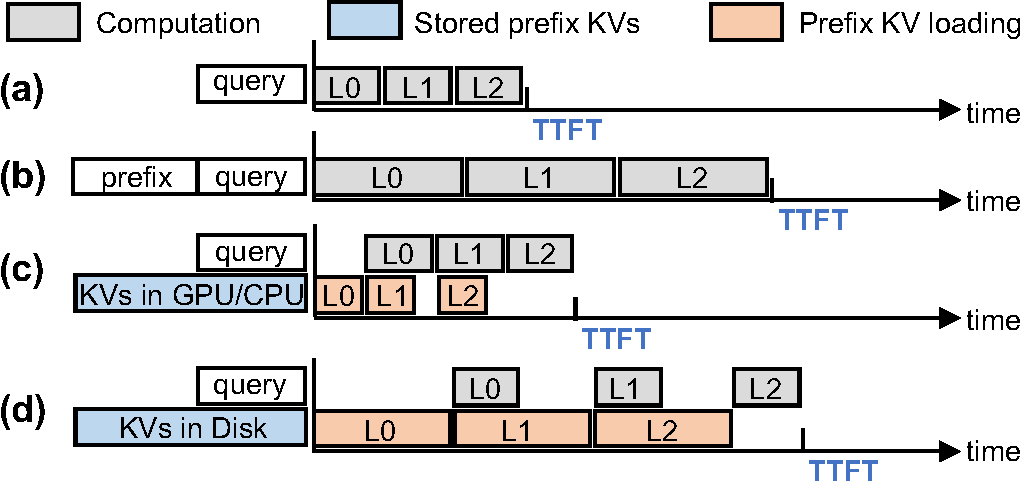
\includegraphics[width=3.4in, height=1.6in]{pkvloading.pdf}
	\vspace{-0.2in}
	\caption{The TTFTs of various cases. Assume the LLM model consists of three transformer layers, denoted as `Lx'.}
	\label{fig:pkvloading}
	\vspace{-0.1in}
\end{figure}

\subsection{Shared Prefixes and Storage System}
\label{sec:iobottleneck}
\noindent \textbf{Long TTFT due to the use of context-rich prefixes.}
Directly using large models for inference can lead to suboptimal results. For instance, when queried about a recent event not included in the model's training data, the model might provide incorrect answers. Additionally, due to issues such as hallucinations, the model's responses might contain inaccurate or misleading information~\cite{siren-arxiv23}. To improve response quality, applications often prepend user \textit{queries} with additional context-rich \textit{prefixes} to form complete \textit{requests}, which are then fed into the LLM as input sequences.
For example, Retrieval-Augmented Generation (RAG)~\cite{rag-nips20} searches external knowledge bases for documents relevant to the user's query. Advanced GPT plugins, such as Chameleon~\cite{chameleon-nips23}, include tool definitions in the system prompt and use few-shot examples to guide the LLM in performing complex reasoning tasks. Multi-turn dialogue applications~\cite{attentionstore-atc24} add previous question-answer pairs to the user's latest query for better intent understanding, while the self-consistency technique~\cite{selfcons-ase23} generates multiple responses to the same query and uses voting to improve accuracy.

Figure~\ref{fig:pkvloading}(a) and Figure~\ref{fig:pkvloading}(b) show that while these context-rich prefixes improve the quality of responses, they also significantly increase the time-to-first-token (TTFT), which is the delay before the model generates the first token. For instance, the Chameleon system adds over 2,600 tokens of context before the user's query~\cite{chameleon-prompt}. Given that the average real-world user query is about 750 tokens~\cite{sharegpt}, this increases the request token count by more than 4$\times$, extending the TTFT by 9$\times$ for the OPT-30B model due to the additional computation. This can negatively impact user experience, especially in TTFT-sensitive applications like real-time chatbots. 
\fv{
Besides, it also degrades the system's overall throughput and increases the enterprise costs.	
}
This paper focuses on reducing TTFT during the prefill phase without altering the decoding phase. Note that shortening TTFT also reduces decoding latency for other requests, as modern systems use continuous batching, where the decoding of existing and newly-arrived requests are processed together after the completion of the prefill of the new requests~\cite{orca-osdi22}.

\noindent \textbf{Prefix KV storage systems and I/O bottleneck.}
Researchers have observed that these prefixes are often partially or completely shared across different requests~\cite{sglang-arxiv23, chunkattention-arxiv24, cachegen-sigcomm24, ragcache-arxiv24, promptcache-mlsys24, attentionstore-atc24}. For example, similar queries might retrieve partially or entirely the same related documents using RAG; the same GPT plugin can be used multiple times, resulting in identical system prompts across requests. 
Recomputing the K and V tensors in Figure~\ref{fig:llm} for the same prefix leads to wasted computational resources and increased TTFT. To optimize TTFT, existing systems store and reuse the K and V tensors of these shared prefixes (referred to as \textit{prefix KV cache} or simply \textit{prefix KV}). Note that the Q tensor of the prefix is not stored, as it is not needed for subsequent computations~\cite{attentionstore-atc24}. When a new request with a repeated prefix arrives, the system asynchronously preloads its prefix KVs into GPU memory, thereby reducing TTFT during the prefill phase of the new request.


\begin{figure}
	\centering
	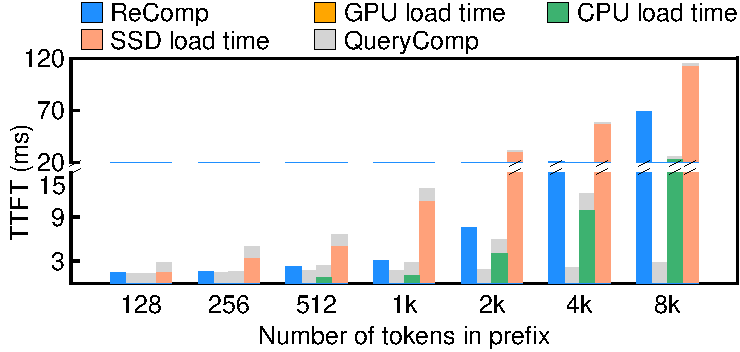
\includegraphics[width=3.3in, height=1.55in]{pload_bottleneck.pdf}
	\vspace{-0.1in}
	\caption{TTFT breakdown.
				`ReComp' refers to not reusing the prefix KV. `QueryComp' denotes the remaining computation after loading the prefix KV. }
%	\vspace{-0.1in}
	\label{fig:pload-bottleneck}
	\vspace{-0.15in}
\end{figure}

\cp{\subsection{Limitations of Existing Approaches}}

An effective prefix KV storage system must meet two requirements. First, it needs sufficient storage capacity to hold enough prefix KVs. A 2,600-token prefix KV alone requires 3.4 GB of storage space for a medium-sized OPT-30B model. Second, the latency for prefetching the prefix KV must be low. Otherwise, it will become a bottleneck of the LLM inference, limiting the reduction of TTFT. 
Currently, no system can simultaneously meet these two requirements across various scenarios.
Most existing systems store prefix KVs only in GPU and/or CPU
memory~\cite{promptcache-mlsys24, sglang-arxiv23, ragcache-arxiv24,
chunkattention-arxiv24}, as shown in Figure~\ref{fig:pkvloading}(c), to reduce
TTFT. However, the limited space in GPU and CPU memory quickly becomes
exhausted. Although the latest prefix KV storage system,
AttentionStore~\cite{attentionstore-atc24}, stores the prefix KV on both CPU
memory and disk to provide sufficient storage space, it doesn’t fundamentally
reduce the load time, as the latency from disk cannot be fully hidden by
computation in some cases as shown in Figure~\ref{fig:pkvloading}(d).  
%Although it asynchronously loads the prefix KVs of upcoming inference requests from disk to CPU memory based on scheduler information, 
Thus, this approach may fail under heavy request loads or in preemptive scheduling scenarios, due to the bottleneck of disk I/O.
%Figure~\ref{fig:pload-bottleneck} shows the TTFT breakdown for recalculating shared prefixes versus loading prefix KV from different storage media using the xx dataset (details in \cref{exp:setup}). Despite the use of asynchronous loading, the I/O time required to load prefix KVs into GPU memory, which cannot be masked by computation, as shown in the figure, can account for x\% to y\% of TTFT, becoming a new bottleneck in inference.
\zrdnew{IMPRESS~\cite{impress-fast25} proposes that loading only important KVs to reduce I/O latency while maintaining comparable accuracy. However, the identification and loading of important KVs for the next layer depend on the computation results of the current layer, which makes it impossible to prefetch them during the current layer's computation. As xxx shows, although this approach reduces the I/O volume, it fails to leverage the opportunity to parallelize I/O with computation, resulting in the I/O bandwidth being underutilized during computation.}
Figure~\ref{fig:pload-bottleneck} shows the TTFT breakdown for recalculating
shared prefixes versus loading and reusing prefix KVs from different storage
media (i.e., GPU memory, CPU memory, and SSD). We vary the number of input prefix tokens from
128 to 8k. The ``load''  time represents the I/O latency that cannot be hidden by
query computation. 
%It demonstrates that while most I/O latency can be hidden when loading prefix KVs from GPU and CPU, loading from SSD results in load stalls, which account for 51\%-98\% of the total TTFT.
It shows that loading prefix KVs from GPU or CPU results in shorter TTFT compared to recomputation, but loading from SSD leads to longer TTFT. This is due to the I/O latency from SSD to GPU, which is rarely hidden by query computation and accounts for 51\%-98\% of the total TTFT.
Consequently, prefix KV loading has become a new bottleneck in model inference, particularly for longer prefixes.



\subsection{Not All KVs Are Equally Important}
Recent research~\cite{h2o-nips23, infinigen-osdi24, flexgen-icml23, scissorhands-nips23} indicates that not all tokens' KVs are equally important for maintaining LLM inference accuracy. These methods generate and store the full set of KVs during the prefill phase, then  identify and discard the less important tokens' KVs during decoding by analyzing the attention weights. This approach reduces the computational load during the decoding phase while maintaining comparable LLM inference accuracy.

Inspired by this, we propose an importance-informed three-tiered prefix KV
\zrd{caching and speculative prefetching system} that encompasses GPU memory, CPU memory, and disk storage. \zrd{Our system addresses the disk I/O bottleneck through a two-pronged approach: selective loading and speculative prefetching. When reusing prefix KVs, we selectively load only important KVs for prefill and decoding computations, while unimportant tokens' KVs are discarded. To further optimize I/O efficiency, we propose a \technew{} mechanism that uses the current layer's important token indices to predict and prefetch the next layer's important KVs during computation, effectively overlapping I/O operations with computation. This integrated approach of selective loading combined with cross-layer speculative prefetching fundamentally alleviates the disk bottleneck by both reducing the total I/O volume and moving critical I/O operations off the inference critical path, thereby significantly reducing TTFT.} 
%When
%reusing prefix KVs, we aim to load only important KVs
%%  rather than fetching them
%% all. 
%% \wj{Only important prefix tokens' KVs participate in prefill and decoding
	%% computations, while unimportant tokens' KVs are discarded.}
%for prefill and decoding computations, while unimportant tokens' KVs are discarded.
%Selectively loading the important KVs can
%fundamentally alleviate the disk
%bottleneck, thereby reducing TTFT.

% when reusing prefix KVs 

